\chapter{Enrichment of SAC proteins at kinetochores strengthens the Spindle Assembly Checkpoint Signaling}
\label{chpt:3}

\section{Recruitment of \protein{BubR1} by \protein{Bub1} \Latin{per se} contributes to the activity of the kinetochore-based SAC signaling}



%Cells rescued with mCherry-\protein{BubR1} (wildtype) have a lower SAC signaling activity than the parental cells treated with the control siRNA, probably due to the lack of control over the expression level of the ectopic mCherry-\protein{BubR1}.

% This observation matched those from \cite{BubBiochem, BubR1TwoPools}.

\protein{BubR1} is mainly recruited to \protein{Knl1} by \protein{Bub1} \cite{BubBiochem,BubR1TwoPools}. As \protein{Bub1} is an important hub protein that binds other SAC proteins (like \protein{Cdc20} and \protein{Mad1} that coordinate to promote the efficient assembly of MCC \Latin{in vitro} and in \Latin{Caenorhabditis elegans} \cite{BUB1-CDC20-MAD1,Tripartite}), we reasoned that \protein{BubR1} recruited to the kinetochores by \protein{Bub1} should facilitate MCC assembly better than free cytosolic \protein{BubR1} does. Our kinetochore-independent experiment using truncations of \protein{Bub1} showed that \protein{BUB1} which is able to bind \protein{BubR1} promotes MCC assembly better than \protein{Bub1} which is unable to bind \protein{BubR1} does (manuscript in preparation). However, previous studies show that either the deletion of the heterodimerization domain of \protein{Bub1} in an in vitro reconstitution system \cite{BUB1-CDC20-MAD1} or the mutation of the GLEBS domain of kinetochore-tethered \protein{Bub1} \cite{MIS12-BUB1-E252K}, both of which abolished the hetero-dimerization between \protein{Bub1} and \protein{BubR1}, has no effect on the SAC signaling activity. Moreover, two previous studies using \protein{BubR1} rescue experiments in nocodazole-treated cells demonstrated that the heterodimerization between \protein{BubR1} and \protein{Bub1} actually shortens the duration of mitotic arrest \cite{BubR1TwoPools,BubBiochem}. Even though the two studies deleted different segments of \protein{BubR1}'s heterdimerization domain which mediates \protein{BubR1}'s interaction with \protein{Bub1} (a.a 440-460 \cite{BubR1TwoPools}, hereafter refer to as ``HD\textsuperscript{short}'', versus a.a. \textDelta{}432-484 \cite{BubBiochem}, hereafter refer to as ``HD'') and used different concentrations (\SI{\sim100}{nM} in \cite{BubR1TwoPools} versus \SI{50}{nM} in \cite{BubBiochem}) of nocodazole to induce signaling kinetochores, the basic observations were consistent, which prompts us to examine the matter carefully.
% which might have resulted in the observation of different levels of heterodimerization domain-truncated \protein{BubR1} remaining at signaling kinetochores

We noted that first, there were no mentioning of rigorous control over the expression level of exogenous \protein{BubR1} to match the physiological level of endogenous \protein{BubR1} in these two studies.
Second, the concentrations of nocodazole used in these two studies allowed the existence of some spindle microtubules \cite{100nMNoc}. However, PP2A's recruitment by \protein{BubR1}'s kinetochore attachment regulatory domain (KARD) to signaling kinetochores is known to contribute to the silencing of the SAC either directly (by dephosphorylating the MELT motif \cite{PP2ADephosphorylatesKNL1} or \protein{Bub1} \cite{PP2ADephosphorylatesBUB1}) or indirectly (by stabilizing the kinetochore-microtubule attachment \cite{Suijkerbuijk2012, BUBR1-L669A+I672A, PP2A-B56-BUBR1ChromosomeCongression_Xu2013} or promoting PP1's recruitment \cite{PP2A-B56}). PP2A's recruitment to signaling kinetochores might not be completely canceled by \protein{BubR1}(\textDelta{}HD)'s defective interaction with B56 \cite{BubBiochem}, RNA interference against B56's (due to probable incomplete knock-down), or mutating \protein{BubR1}'s KARD (\cite{BubR1TwoPools}, which eliminated the binding of the B56\textalpha{} isoform \cite{BUBR1-L669A+I672A}). Third, although the depletion of \protein{BubR1} does not affect the localization of \protein{Cenp-E} at signaling kinetochores in HeLa cells \cite{CENPELocalization-BUBR1}, the activity of kinetochore-localized \protein{Cenp-E}
% (to facilitate transition of spindle microtubule-kinetochore attachment from lateral attachment into end-on attachment)
may be affected by the loss of interaction with \protein{BubR1} \cite{CENPEActivity-BUBR1} when cells are rescued by heterodimerization domain-truncated \protein{BubR1}, which may affect chromosome congression.
% \protein{BubR1} is known to interact with \protein{Cenp-E} which facilitates chromosome alignment, and may arguably regulate the activity of kinetochore-localized \protein{Cenp-E} \cite{CENPELocalization-BUBR1, CENPEActivity-BUBR1}. However, the potentially reduced \protein{Cenp-E} activity at the kinetochore in mNG-\protein{BubR1}(\textDelta{}HD, \textDelta{}KARD)-rescued cells should only result in an increased SAC response, compared to mNG-\protein{BubR1}(\textDelta{}KARD)-rescued cells.

%Therefore, we designed and performed new \protein{BubR1} rescue experiments with the help of our CRISPR-Cas9-edited mNG-\gene{BubR1} cell line.
Therefore, we decided to compare the SAC activity of BUBR1(\textDelta{}KARD) and BUBR1(\textDelta{}KARD, \textDelta{}HD). The truncation of KARD (a.a. 665-682) abolishes the binding of B56\textalpha{} \cite{Suijkerbuijk2012} and likely other isoforms of B56 onto BUBR1 as well \cite{B56-SLiM, PP2A-B56-BUBR1Structure}, which allow us to dissect whether the recruitment of BUBR1 to the signaling kinetochore per se contributes to the SAC activity. Additionally, mNG-\protein{BubR1}(\textDelta{}HD, \textDelta{}KARD) lacks the heterodimerization domain (HD). Indeed, mNG-\protein{BubR1}(\textDelta{}HD, \textDelta{}KARD) does not have identifiable localization at signaling kinetochores \cite{BubBiochem} (\myref{BUBR1del432-484KTLocalization}). The mitotic arrest was induced by treatment with \SI{25}{nM} of nocodazole \cite{25nMNoc} after thymidine release, where unattached kinetochores can be observed while metaphase plates remain largely intact (\myref{BUBR1del432-484KTLocalization}) . Control siRNA-treated mNG-\gene{BubR1} HeLa-A12 cell line was imaged under the same condition to provide a reference for the physiological expression level of endogenous \protein{BubR1}. Only mitotic cells having $0.5\times$ -- $2\times$ the average mNeonGreen intensity of mNG-\gene{BubR1} HeLa-A12 cells during mitosis were included in the analysis (noted that only about half of endogenous \protein{BubR1} proteins are tagged in the CRISPR-Cas9-edited cell line).

\begin{figure} [b!]
    \centering
    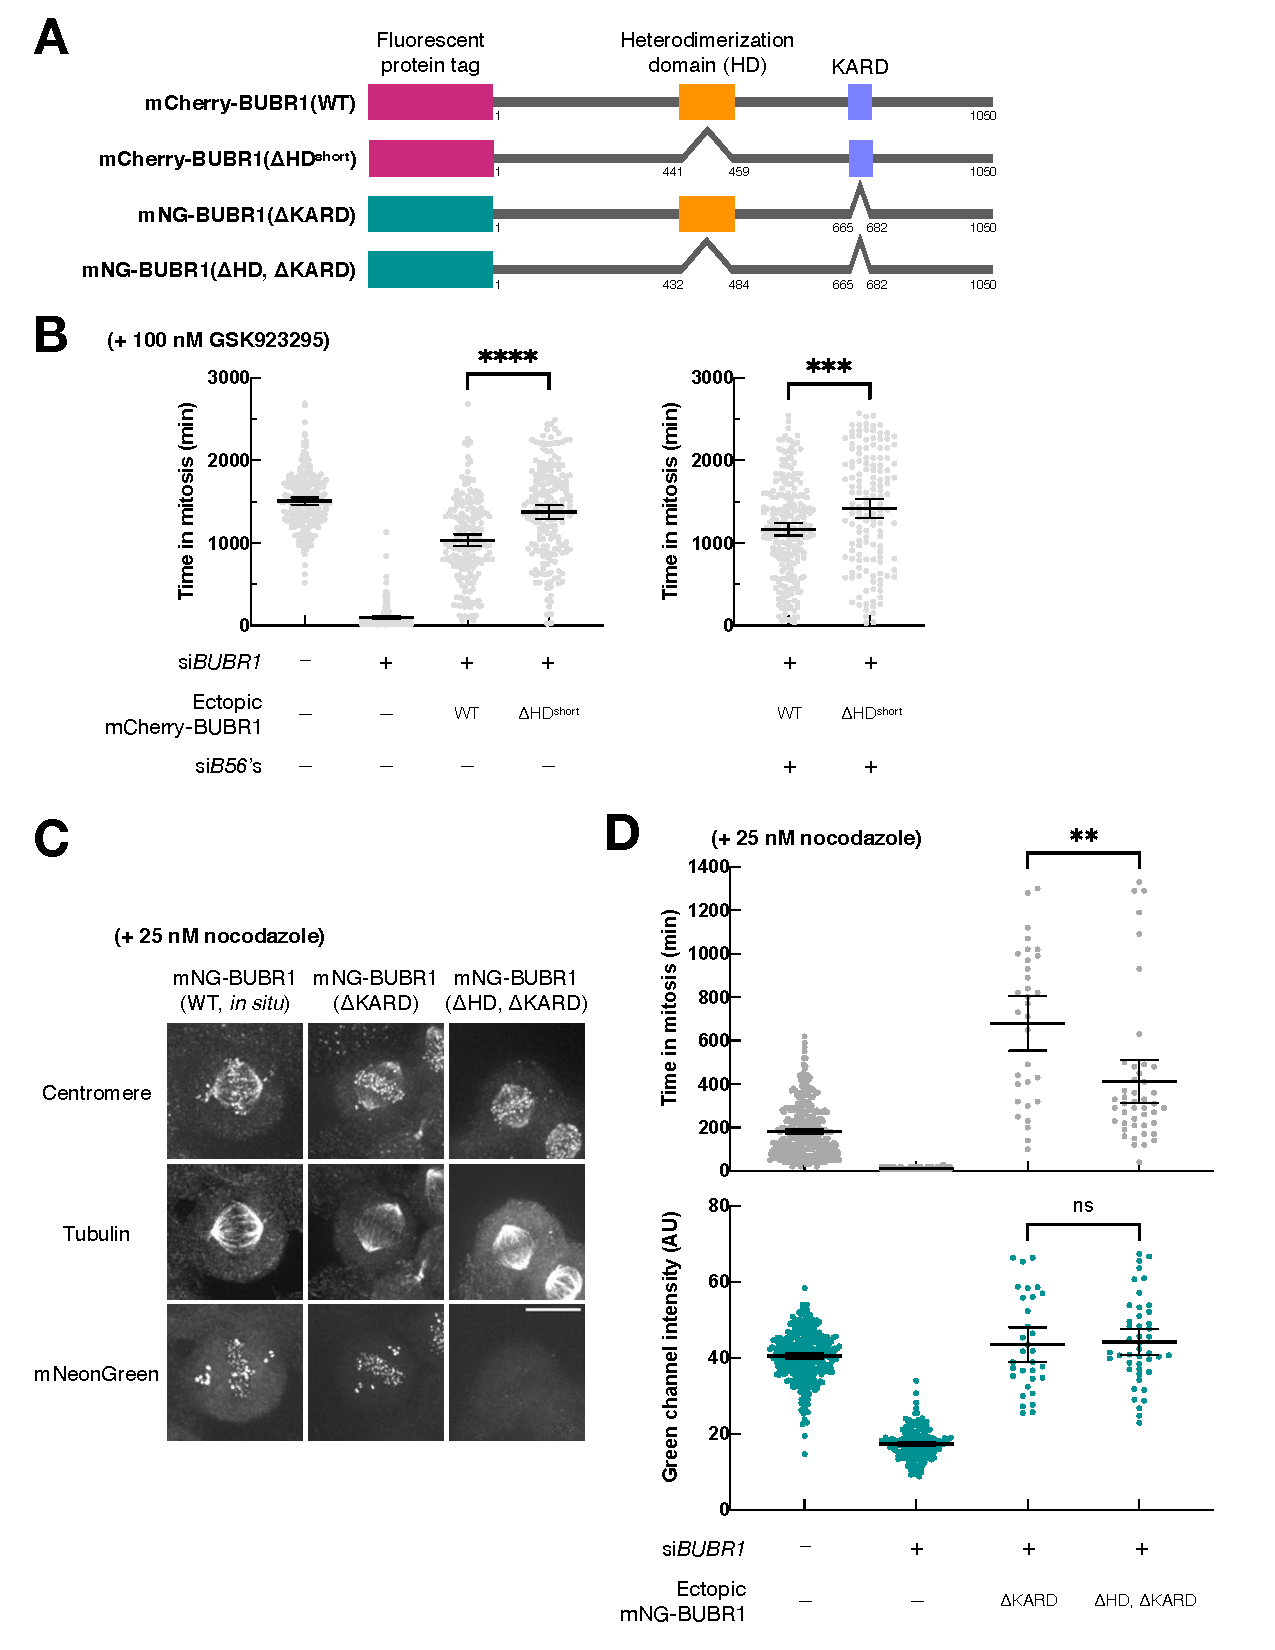
\includegraphics[width=\textwidth]{chapters/figures/RescueExperiment.pdf}
    \phantomsubfiglabel{RecombinantBUBR1Diagram} % subfigure A
    \phantomsubfiglabel{OldBUBR1Rescue} % subfigure B
    \phantomsubfiglabel{BUBR1del432-484KTLocalization} % subfigure C
    \phantomsubfiglabel{NewBUBR1Rescue} % subfigure D
    \caption{\textbf{Recruitment of \protein{BubR1} by \protein{Bub1} to signaling kinetochores \Latin{per se} contributes to the SAC signaling activity.}}
    \label{RescueExperiment}
\end{figure}
\addtocounter{figure}{-1}
\begin{figure} [t!]
  \noindent\justifying \textbf{(Caption of \myref{RescueExperiment} continued from the previous page)} \textbf{(A)} Diagrams (not to scale) of all ectopic recombinant BUBR1's used in experiments associated with \myref{OldBUBR1Rescue,BUBR1del432-484KTLocalization,NewBUBR1Rescue}. \textbf{(B)} A \gene{BubR1} knockdown-rescue experiment with mCherry-\protein{BubR1} or mCherry-\protein{BubR1}(\textDelta{}HD\textsuperscript{short}) (with an HD truncation from \cite{BubR1TwoPools}). \cite{BubR1TwoPools} uses a shorter HD truncation compared to \cite{BubBiochem}. Therefore, it is denoted as \textDelta{}HD\textsuperscript{short} here. We used \SI{100}{nM} GSK923295 to activate the SAC signaling, which is different from both \cite{BubR1TwoPools} (\SI{100}{nM} nocodazole) and \cite{BubBiochem} (\SI{50}{nM} nocodazole). Cells rescued with mCherry-\protein{BubR1} consistently have a lower SAC signaling activity than cells rescued with mCherry-\protein{BubR1}(\textDelta{}HD\textsuperscript{short}), no matter whether B56's were knocked down. Each dot represents a cell, with more than 140 cells in each group. Unpaired $t$-tests with Welch's correction were performed in Prism 9. Frank Ferrari also contributed to the data analysis here. \textbf{(C)} Confocal immunofluorescence images (by Dr. Ajit Joglekar) showed that \SI{25}{nM} nocodazole impaired the congression of a few chromosomes (which activated the SAC) %but left the spindles largely intact
  in both genome-edited mNG-\gene{BubR1} HeLa A12 (the first column) and the RMCE HeLa A12 (the second and the third columns). In the second and the third columns, RMCE HeLa A12 cells were treated with si\gene{BubR1} and \SI{0.5}{\micro g/mL} of doxycycline to induce the ectopic expression of indicated mN-\protein{BubR1} variants. Ectopically expressed mNG-\protein{BubR1}(\textDelta{}HD, \textDelta{}KARD) could not be detected at kinetochores (the third columns) while mNG-\protein{BubR1}(\textDelta{}KARD) could. Maximum $z$-projections of representative cells were shown for each condition (column) and channel (row). The LUTs for the mNeonGreen channel are the same across different conditions. Scale bar, \SI{10}{\micro m}. \textbf{(D)} A \gene{BubR1} knockdown-rescue experiment with mNG-\protein{BubR1}(\textDelta{KARD}) or mNG-\protein{BubR1}(\textDelta{}HD, \textDelta{}KARD) (with an HD truncation from \cite{BubBiochem}). Top panel: the mitotic duration of individual cells. Bottom panel: the cytosolic mNeonGreen signal of individual cells. In the heterozygous, genome-edited mNG-\gene{BubR1} HeLa A12 (first two columns), both the wildtype allele and the edited mNG-\gene{BubR1} allele are susceptible to si\gene{BubR1}. In the RMCE HeLa A12 cells (last two columns), ectopically expressed mN-\protein{BubR1} variants are resistant to si\gene{BubR1}. Each dot represents a cell, with more than 30 cells in each group. Results are representative of two independent experiments. Unpaired $t$-tests with Welch's correction were performed in Prism 9.
\end{figure}

According to the average duration from the NEBD to the anaphase onset, The knockdown of \gene{BubR1} is efficient enough to almost completely abolish the SAC. mNG-\protein{BubR1}(\textDelta{}KARD)-rescued cells. mNG-\protein{BubR1}(\textDelta{}KARD)-rescued cells take longer in mitosis than the control group, which is consistent with previous studies and can be explained by increased phosphorylation of \protein{Knl1} and/or attenuated kinetochore-microtubule attachment \cite{PP2A-B56, BUBR1-L669A+I672A}. Most importantly, in contrast to previous findings, our final data showed that mNG-\protein{BubR1}(\textDelta{}KARD)-rescued cells take longer in mitosis than mNG-\protein{BubR1}(\textDelta{}HD, \textDelta{}KARD)-rescued cells do (\myref{NewBUBR1Rescue}), directly supporting that the recruitment of \protein{BubR1} \Latin{per se} contributes to the activity of the kinetochore-based SAC signaling.

\protein{BubR1} interacts with the kinase \protein{Plk1}, a key regulator throughout mitosis \cite{BUBR1-PLK1}. It should be noted that mNG-\protein{BubR1}(\textDelta{}KARD) may still recruit \protein{Plk1}, while mNG-\protein{BubR1}(\textDelta{}HD, \textDelta{}KARD) itself does not localize to signaling kinetochores. Although depletion of \protein{BubR1} only results in a marginal reduction of \protein{Plk1} at signaling kinetochores \cite{CENPU+BUB1-PLK1}, it remains to be examined how much the discrepancy in the localization of \protein{Plk1} contributes to our our results here.


\section{Materials and Methods}
\subsection{CRISPR-Cas9 mediated genome editing and cell culturing}
The guide RNAs (gRNAs) for \Latin{in situ} \gene{BubR1} and \gene{Bub1} N-terminal mNeonGreen-tagging were \Oligo{caggauggcggcggugaaga}
% #20
and \Oligo{gguucagguuuggccgcugc},
%#9 \Oligo{gguucagguuuggccgcugc}
respectively. The gRNA for \Latin{in situ} \gene{Mad1}
%and \gene{CcnB1}
C-terminal mNeonGreen-tagging was \Oligo{cagaccguggcguagccugc}.
%and \Oligo{GAUCUUAGCAUGCUUCGAUG}, respectively
Single guide RNAs (sgRNAs) were synthesized using the EnGen sgRNA Synthesis Kit (for the \Latin{Streptococcus pyogenes}-originated Cas9, New England Biolabs). The \Latin{Sp}Cas9-sgRNA ribonucleoprotein (RNP) complex was assembled at room temperature in a buffer consisting of 20 mM of HEPES-KOH (pH 7.5), 150 mM of KCl, 1 mM of MgCl$_2$, 10\% (by volume) of glycerol, and 1 mM of DTT using 100 pmol of \Latin{Sp}Cas9-$2\times$NLS (the QB3 MacroLab) and 120 pmol of sgRNA. The RNP complex and \SI{1.5}{\micro g} of the corresponding linearized homology-directed repair template plasmid were co-transfected into $2\times 10^5$ -- $5\times 10^5$ nocodazole-arrested mitotic HeLa A12 cells \cite{CRISPRProtocol} (harvested by the mitotic shake-off method) using the Cell Line Nucleofector\texttrademark{} Kit R (Lonza) following manufacturer's instructions. After one week, green fluoresence-positive mitotic cells (arrested by 330 nM nocodazole for 16 h) were sorted directly into 96-well plates at 1 cell/well. Healthy colonies were subject to further validation by fluorescence imaging, genotyping and sequencing, as well as immunoblotting.

All HeLa-A12 cells were cultured in DMEM (with high glucose and phenol red, without glutamine, sodium pyruvate, or HEPES; Gibco) supplemented with 22 mM of HEPES (Corning), 9\% (by volume) of fetal bovine serum (Corning), and $1\times$ GlutaMAX (Gibco). For Cre-Lox recombination-mediated cassette exchange, Lipofectamine 3000 (Invitrogen) is used to co-transfect \SI{1.5}{\micro g} of a circular plasmid carrying the transgene cassette and \SI{50}{ng} of the circular pCAGGS-nlCre plasmid. \SI{0.5}{\micro g/mL} of puromycin was added 1.5 d later for 3 d to select for stably-transfected HeLa-A12 cells. Puromycin-resistant colonies were then pooled together and subject to further validation by genotyping (data not shown).
%and/or immunoblotting

Successfully-edited alleles encode mNeonGreen-tagged SAC proteins that separate the corresponding wildtype protein and the fluorescent protein mNeonGreen by a short flexible linker (mNG-\protein{BubR1} and mNG-\protein{Bub1}: \Peptide{GSGGSG}; \protein{Mad1}-mNG: \Peptide{GGAGGSGG}). Exact sequences of all homology-directed repair template plasmids and Cre-Lox recombination-mediated cassette exchange plasmids (encoding \protein{Spc25}-mCherry, \protein{Knl1}\textsuperscript{\textDelta{}}-M3, or \protein{Knl1}\textsuperscript{\textDelta{}}-M3-M3 transgenes) are available upon request.

\subsection{Genotyping}
HeLa-A12 genomic DNAs were purified using the Wizard SV Genomic DNA Purification System (Promega). Genotyping primers (\gene{BubR1} forward primer \Oligo{cctggtcacatctgagctat},
% cctggtcacatctgagctat 1942 ?
\gene{BubR1} reverse primer \Oligo{ctcagtgagactccagtgtt},
% ctcagtgagactccagtgtt 1943 ?
\gene{Bub1} forward primer \Oligo{ccctctacatgaaggcgcta},
% ccctctacatgaaggcgcta 2082 ? 
\gene{Bub1} reverse primer \Oligo{gctcgcccaaggtaaacatt},
% gctcgcccaaggtaaacatt 2083 ?
\gene{Mad1} forward primer \Oligo{ GGACTTTTCAGGGACGTGGT},
% GGACTTTTCAGGGACGTGGT 2094 ?
and \gene{Mad1} reverse primer \Oligo{GAGTTGGGAGGAGGGGACTC})
% GAGTTGGGAGGAGGGGACTC 2093 ?
were designed to bind outside of homology arms to avoid false-positive colonies from integration of the homology-directed repair template plasmid to an off-target genomic locus.

\subsection{Rapid amplification of cDNA ends (RACE)}
Interphase samples were arrested in \SI{2.5}{mM} of thymidine for 1 day and then harvested by trypsinization. Mitotic samples were arrested in \SI{2.5}{mM} of thymidine for 1 day, released into \SI{100}{ng/mL} of nocodazole for 19 h, and finally harvested by mitotic shake-off. Harvested cells were snap-frozen by liquid nitrogen and stored at \SI{-80}{\celsius} until total RNA extraction.

Total RNA extraction was done using the Monarch Total RNA Miniprep Kit (New England Biolabs) following manufacturer’s instructions. The reverse transcription (RT) was done using the Template Switching RT Enzyme Mix (New England Biolabs) following manufacturer’s instructions. The sequence of the template switching oligo (TSO) is \MixedOligo{GCTAATCATTGCAAGCAGTGGTATCAACGCAGAGTACATrGrGrG}. The sequence of the \gene{Bub1}-specific RT reverse primer is \Oligo{ctctgaaggacagcactggcat} (binds to the fourth exon of \gene{Bub1}).

The reverse transcription products were subsequently amplified by nested PCR. The TSO-specific forward primer (incoporating an \textit{Spe}I restriciton site at the 5' end) is \Oligo{GGACTAGTTGCAAGCAGTGGTATCaac}. The \gene{Bub1}-specific reverse primer (incoporating an \textit{Xho}I restriciton site at the 3' end) is \Oligo{TATACTCGAGctctccttgggcttccagat}, which binds to the fourth exon of \gene{Bub1} as well but upstream of the RT reverse primer.

RT-PCR products were visualized on an agarose gel. Individual bands were cut off and purified from the gel, and finally cloned into pBlueScript-KS(+) between the \textit{Spe}I site and the \textit{Xho}I site. For each band, multiple clones were randomly picked for sequencing.

\subsection{Fluorescence correlation spectroscopy (FCS)}
The total number of fluorophores in a homogeneous solution is $N_\text{total} := N_\text{A}cV_\text{total}$, where $N_\text{A}$ is the Avogadro constant, $c$ is the molar concentration of the fluorophore, and $V_\text{total}$ is the total volume of the solution. The probability that a specific fluorophore molecule is within the excitation volume $V_0 (\ll V_\text{total})$ at any given time is
$p_0 := V_0/V_\text{total}\ll1$. For freely diffusive fluorophores in a diluted solution, whether or not a specific fluorophore is within the excitation volume is independent of each other. Thus, the number of fluorophores inside the excitation volume at any given time $N_0$ has a binomial distribution $B(N_\text{total}, p_0)$. Therefore,
\begin{equation*}
    G_0 \coloneqq \dfrac{\sigma_{N_0}^2}{\langle N_0 \rangle^2} = \dfrac{1-p_0}{N_\text{total}p_0} \approx \dfrac{1}{N_\text{A}cV_0}.
\end{equation*}
Under a fixed live-cell imaging setup [which includes the microscope (its alignment and the objective), the wavelength of the excitation light, the thickness of the coverslip (affecting the actual working distance), and the refractive index of the cytosol], $V_0$ is fixed. Therefore, $G_0$ is inversely proportional to the molar concentration of the fluorophore. The average number (or the variance of the number) of fluorophores inside the excitation volume observed over a long period of time should be close to the theoretical mean $\langle N_0 \rangle$ (or the theoretical variance $\sigma_{N_0}^2$).

All FCS data were collected on an Alba v5 Laser Scanning Microscope (ISS), connected to an Olympus IX81 inverted microscope main body [equipped with a UPLSAPO60XW objective (1.2 NA, Olympus)]. A Fianium WL-SC-400-8 laser (NKT Photonics) with an acousto-optical tunable filter was used to generate excitation pulses at a wavelength of \SI{488}{nm} and a frequency of around \SI{20}{MHz}. Excitation light was further filtered by a Z405/488/561/635rpc quadband dichroic mirror (Chroma). Emission went through a 655DCSPXR shortpass dichroic mirror (Chroma) and an FF01-531/40-25 filter (Semrock) and was finally detected by an SPCM-AQRH-15 avalanche photodiode (Perkin Elmer). The time-correlated single photon counting electronics to register detected photon events in relation to the excitation pulses was SPC-830 (Becker \& Hickl). Data acquisition was facilitated by VistaVision (ISS). The excitation volume ($V_0$) was calibrated by taking FCS data from TetraSpeck\texttrademark{} microspheres (\SI{0.1}{\micro m}, Invitrogen) of known concentrations (vary across different batches).

\subsection{RNA interference}
Cells were transfected with siRNA in the morning. 2.5 mM of thymidine was added 8 h later and cells were incubated overnight. The next morning, cells were released from the thymindine block into fresh media. This sequence was then repeated once again and cells were released into FluoroBrite\texttrademark{} DMEM (Gibco) supplemented with 9\% (by volume) of fetal bovine serum and $1\times$ GlutaMAX and incubated for 6 h before the addition of mitotic drugs. Drugs were left to take effect for 1 h before imaging.

Sense-strand sequences and working concentrations of small interfering RNA duplexes (siRNAs) used in this study include the \gene{BubR1} siRNA (\Oligo{GAUGGUGAAUUGUGGAAUA}, 40 nM \cite{siBUBR1}), \gene{Bub1} siRNA (\Oligo{CGAAGAGUGAUCACGAUUU}, 40 nM \cite{BUB1-si5}), and the \gene{ZW10} siRNA (\Oligo{UGAUCAAUGUGCUGUUCAA}, 100 nM \cite{siZW10}). The siRNAs against all five B56 isoforms were taken from the second pool in \cite{siB56s}.
%the \gene{Knl1} siRNA (\Oligo{CACCCAGUGUCAUACAGCCAAUAUU},
%       CACCCAGUGUCAUACAGCCAAUAUU HSS183683
%40 nM \cite{KI2014}).
Desalted siRNA duplexes modified by double-dexoxythymidine overhangs at 3'-ends of both strands were synthesized by Sigma. The AllStars Negative Control siRNA (QIAGEN) was used as the control. All siRNAs were transfected into the cells via Lipofectamine RNAiMAX (Invitrogen) following manufacturer’s instructions.

\subsection{Live-cell imaging}
Cells were plated in a Nunc Lab-Tek II chambered coverglass (Thermo Scientific) or a 35-mm coverglass-bottomed dish (MatTek) and treated with drugs and/or siRNAs accordingly. For imaging, the chambered coverglass or the coverglass-bottomed dish was loaded into a CU-501 temperature and gas control system (Live Cell Instrument). The sample holder was maintained at \SI{37}{\celsius} and ventilated by humidified 5\% of \ch{CO2} and the objective was maintained at \SI{37}{\celsius} by a heating band.

Most $z$-stack imaging (except the measurement of FRET efficiency of MPS1sen-KT) was performed on a Nikon Eclipse Ti-E/B inverted microscope, with a CFI Plan Apochromat Lambda $100\times$, 1.45 NA oil objective (Nikon). The microscope was equipped with an H117E1 motorized stage (Prior Scientific) and a NanoScanZ 100 piezo stage (Prior Scientific). A SPECTRA 5-LCR-XA Light Engine (Lumencor) served as the excitation light source. The 475 nm-centered band of excitation light was used for the green channel and the 575/30-nm-filtered band of excitation light was used for the red channel. An ET-EGFP/mCherry filter cube (Chroma Technology) was used as the dichroic mirror, where the built-in emission filter on the cube has been removed. Emission light in the red channel was filtered by an ET632/60m (Chroma Technology). Emission light in the green channel was filtered by an ET525/50m (Chroma Technology). Emission filters were mounted on a high-speed filter wheel (Prior Scientific) positioned in the light path before the iXon3 EMCCD camera (Andor Technology) operating in the conventional CCD mode. Signaling kinetochores in GSK923295-treated cells were identified by their polar positioning and the enrichment of localized SAC proteins on them.

The FRET measurement with MPS1sen-KT was also performed on a Nikon Eclipse Ti-E/B inverted microscope, with a CFI Plan Apochromat VC $100\times$, 1.40 NA oil objective (Nikon). The microscope was equipped with an H117E1 motorized stage (Prior Scientific), a NanoScanZ 100 piezo stage (Prior Scientific), and an X-Light V2 L-FOV confocal unit with \SI{60}{\micro m} pinholes (CrestOptics). A CELESTA Light Engine (Lumencor) served as the excitation laser source. The 477-nm line (at $25\%$ power with an exposure time of \SI{400}{ms} for each frame) was used for both the green and the FRET channels and the 546-nm line (at $50\%$ power with an exposure time of \SI{400}{ms} for each frame) was used for the red channel. A ZT488/543rpc (Chroma Technology) was used as the dichroic mirror. Emission through both the red and the FRET channels was filtered by an ET605/52m (Chroma Technology) while emission through the green channel was filtered by an ET525/36m (Chroma Technology). Images were acquired by a Prime 95B 25mm sCMOS camera (Teledyne Photometrics). Custom MATLAB programs \cite{HeLaFRETGUI} were used to quantify kinetochore-localized fluorescence signals.

Certain time-lapse live-cell imaging was performed on an ImageXpress Nano Automated Imaging System (Molecular Devices). A SOLA Light Engine (Lumencor) served as the excitation light source. Cells were plated on 24-well cell imaging plates (black plate with treated glass bottom, Eppendorf) and treated with drugs and/or siRNAs accordingly. Input humidified $5\%$ \ch{CO2} flow was maintained at around \SI{19}{psi} and the environment chamber was maintained at \SI{37}{\celsius}. All SAC proteins tagged by mNeonGreen in this paper (\protein{BubR1}, \protein{Bub1}, and \protein{Mad1}) feature inhomogeneous distributions between the cytosol and the nucleus/nuclear envelope in the prophase (data not shown). In principle, they can indicate the accurate timing of the nuclear envelope breakdown (NEBD) in each cell during the time-lapse imaging. However, due to the resolution limit and for consistency, we determined mitotic duration mainly based on cell morphology (from rounding-up at the NEBD to elongation at the anaphase onset) from transmitted-light images. Unless specified otherwise, this quantification was facilitated by a custom semi-automatic MATLAB program \cite{My2019Paper}.
% (source codes are available upon request).

\subsection{Quantification of the F{\"{o}}rster Resonance Energy Transfer (FRET) based on localized fluorescence signals of MPS1sen-KT}
Under fixed fluorescence microscopy settings of a given channel [the excitation line and its power, exposure time, optical components (including the objective, filters, dichroic mirrors, the confocal spinning disk, and the detector) in the light path and their alignment, etc.], the kinetochore-localized fluorescence signal (digital readout) should be proportional to the number of localized mature fluorescence proteins. The coefficients are designated as $g$ and $r_x$ for mNeonGreen and mScarlet-I using the excitation light for mNeonGreen, respectively (the subscript ``x'' stands for cross-excitation 
as mScarlet-I is excited by the excitation light for mNeonGreen here). The number of unbleached mature mNeonGreen and mScarlet-I molecules at a given kinetochore are $G$ and $R$, respectively. While measuring FRET using the excitation light for mNeonGreen and optics settings to detect the emission of mScarlet-I, the bleed-through coefficient of mNeonGreen's fluorescence is designated as $\beta$. Under a FRET efficiency of $\varepsilon$ $(0 \leq \varepsilon \leq 1,$ which describes the quenching of mNeonGreen due to FRET), the proximity ratio $\Theta$, a metric of FRET according to the definition in \cite{HeLaFRETGUI}, can be expressed as
\begin{equation*}
    \Theta := \dfrac{F}{r_xR + \beta gG(1 - \varepsilon)} - 1,
\end{equation*}
where $F$ is the measured raw FRET readout. $F$ can be attributed to three sources: (1) the cross-excitation of mScarlet-I, (2) the bleed-through of mNeonGreen's fluorescence, and (3) the actual fluorescence due to FRET (determined by the combined coefficient $f$ for excited fraction of mNeonGreen under the excitation condition of the FRET channel and the conversion from FRET emission photons reaching the detector to digital readout, the FRET efficiency $\varepsilon$, and the effective quantum yield $\phi$ of mScarlet-I that reaches the detector).
\begin{equation*}
    F = r_xR + \beta gG(1 - \varepsilon) + fG\varepsilon\phi
\end{equation*}
In \cite{MPS1senor}, the authors used the ratio between the mNeonGreen signal (measured from the green channel) and the raw FRET signal (without corrections of the cross-excitation of mScarlet-I and the bleed-through of mNeonGreen's fluorescence) as the metric of FRET:
\begin{equation*}
    \Gamma := \dfrac{gG(1 - \varepsilon)}{F}.
\end{equation*}
Because MPS1sen-KT competes with endogenous \protein{Spc24} to get recruited to the outer kinetochore region, the number of kinetochore-localized sensors is variable for different kinetochores. However, the ratio between kinetochore-localized mNeonGreen and mScarlet-I is always $1 : 1$. Ignoring photobleaching (only one $z$-stack is taken for each cell with a bare minimum amount of exposure) and assuming that maturation of mNeonGreen and mScarlet-I is independent of the kinases' or phosphatases' activity at kinetochores, $\sigma := R/G$ should also be fixed. Hence, we have
\begin{align*}
    \Theta &= \dfrac{f\varepsilon\phi}{r_x\sigma + \beta g(1 - \varepsilon)},\\
    \Gamma &= \dfrac{g(1 - \varepsilon)}{r_x\sigma + \beta g(1 - \varepsilon) + f\varepsilon\phi}.
\end{align*}
Importantly, both $\Theta$ and $\Gamma$ are dimensionless metrics normalized against the variation in the kinetochore localization of MPS1sen-KT. Under a particular fluorescence microscopy setting, both $\Theta$ and $\Gamma$ have a monotonic and hyperbolic relationship with the FRET efficiency and are interconvertible:
\begin{equation*}
    \Theta = \dfrac{g(1 - \varepsilon)}{r_x\sigma + \beta g(1 - \varepsilon)}\cdot\dfrac{1}{\Gamma} - 1.
\end{equation*}

\subsection{Immunoblotting}
To acquired unsynchronized HeLa-A12 cells, cells were either scrapped or trypsinized off the surface of dishes. To acquired mitotic HeLa-A12 cells, cells were first synchronized in G1/S with \SI{2.5}{mM} thymidine and then arrested in mitosis with \SI{330}{nM} of nocodazole for \SI{16}{h} before mitotic shake-off. Shook-off mitotic cells were then washed once by phosphate buffered saline (Gibco), pelleted down, and chilled on ice. Lysis was performed by directly adding $2 \times$ Laemmli sample buffer (supplemented by 2-mercaptoethanol, Bio-Rad Laboratories) at a ratio of \SI{1}{\micro L} per \SI{0.1}{mg} of cell pellets and pipetting up and down. Lysates were boiled immediately afterwards for \SI{10}{min} and then chilled on ice.
% \SI{8}{\micro L} of supernatant was loaded onto each lane of a 15-well, 0.75-mm SDS-PAGE mini gel.
Primary antibodies (and their working dilution factors by volume) used included anti-\protein{BubR1} (Bethyl Laboratories A300-995A, $1 : 1000$), anti-\protein{Mad1} (GeneTex GTX109519, $1 : 2000$), anti-\protein{Cdc20} (Santa Cruz Biotechnology sc-13162, $1 : 200$), anti-\protein{Bub3} (Sigma-Aldrich B7811, $1 : 500$), anti-mNeonGreen (ChromoTek 32F6, $1 : 500$), anti-GAPDH (Proteintech 60004-1-Ig, $1 : 5000$), anti-\protein{Bub1} (three antibodies purified from different hosts were used: (1) Bethyl Laboratories A300-373A, $1 : 330$, rabbit polyclonal antibody; (2) SB1.3 \cite{SheepAntiBUB1}, $1 : 1000$, sheep polyclonal antibody; (3) Abcam ab54893, $1 : 200$, mouse monoclonal antibody), and anti-DsRed2 (Santa Cruz Biotechnology sc101526, $1 : 5000$).